\section{训练原理}
\subsection{评价指标}
\subsubsection{交叉熵损失函数与准确率}
为全面评估模型在 LaTeX 序列生成过程中的训练效果与预测性能，引入损失层面与性能层面的两类指标：
交叉熵损失（Cross-Entropy Loss，以整数标签为输入）与逐词元准确率（Token-Level Accuracy）。
前者作为优化目标，衡量每个位置上预测分布与真实标签之间的差异；
后者作为性能指标，统计生成序列中预测词元与参考词元的匹配情况，从而反映模型在序列级别的预测精度。
\begin{enumerate}[label={（\arabic*）}, leftmargin=2em, labelsep=0.5em, itemsep=0pt]
    \item 交叉熵损失函数：
    模型在某一时间步的输出为 logit 向量 $\boldsymbol{z} = [z_0, z_1, \dots, z_{C-1}]$，其中 $C$ 为类别总数，$z_j$ 表示第 $j$ 类的预测得分（未归一化），真实标签为 $y \in \{0, 1, \dots, C{-}1\}$。则该时间步的交叉熵损失定义为：
    \begin{equation}
    \mathcal{L}_{\text{CE}} = -\log \left( \frac{e^{z_{y}}}{\sum_{j=0}^{C-1} e^{z_j}} \right) = -z_{y} + \log\left( \sum_{j=0}^{C-1} e^{z_j} \right)
    \end{equation}
    上式右端将 Softmax 与负对数似然合并为对数-求和-指数（log-sum-exp）形式，可直接以未归一化的 logits 计算，避免显式指数运算导致的上溢／下溢等数值不稳定问题。该损失函数在 PyTorch 中通过如下函数实现：
    \begin{center}
        \texttt{torch.nn.functional.cross\_entropy(logits, labels)}
    \end{center}
    其中 \texttt{labels} 为整数编码的真实标签张量，\texttt{logits} 为模型输出的未归一化得分张量；
    该实现内部融合了 log-softmax 与负对数似然计算，保证数值稳定性。
    \item 准确率：
    准确率用于衡量模型在所有预测位置上分类正确的比例。模型在每个位置的预测类别为：
    \begin{equation}
    \hat{y} = \arg\max_{j} z_j
    \end{equation}
    整体准确率定义为：
    \begin{equation}
    \text{Accuracy} = \frac{1}{N} \sum_{i=1}^{N} \mathbb{I}[\hat{y}_i = y_i]
    \end{equation}
    其中 $\mathbb{I}[\cdot]$ 为指示函数，表示预测是否正确，$N$ 为所有评估位置的总数。
\end{enumerate}
\subsubsection{掩蔽损失函数与掩蔽准确率}
    为满足批量训练对张量形状一致性的要求（解码器的位置嵌入亦需预设固定的最大长度），需对标签序列进行填充，统一长度至最大值。填充标记通常为特殊符号 \texttt{<PAD>}，其对应的标签值设为 $0$。为避免这些填充位置对损失计算与评估指标造成干扰，引入掩蔽机制，在损失与准确率计算中仅考虑非填充位置。
    加权平均的掩蔽交叉熵损失函数定义如下：
    \begin{equation}
    \mathcal{L}_{\text{masked}} = \frac{\sum_{i=1}^{L} m_i \cdot \mathcal{L}_i}{\sum_{i=1}^{L} m_i}, \quad
    m_i =
    \begin{cases}
    1, & \text{若 } y_i \neq 0 \text{ 且 } \mathcal{L}_i < 10^8 \\
    0, & \text{否则}
    \end{cases}
    \end{equation}
    其中，$L$ 表示序列长度，$y_i$ 为第 $i$ 个时间步的真实标签，$\mathcal{L}_i$ 为其对应的单步交叉熵损失，$m_i$ 为掩码指示变量。仅当 $y_i$ 为有效标签（非 \texttt{<PAD>}）且 $\mathcal{L}_i$ 不出现数值异常时，才将该位置纳入最终损失计算。
    掩蔽准确率同样排除填充位置，仅在非填充位置统计预测是否正确；与掩蔽损失不同的是，准确率\textbf{不}额外排除 $\mathcal{L}_i \ge 10^8$ 的位置，故测试集中被映射为 \texttt{[UNK]} 的词表外（OOV）目标位置仍计入统计——由于 \texttt{[UNK]} 在输出层被一项词频先验偏置（其设计见“模型构建”一章的 TokenOutput 层）禁止生成，这些位置必然计为错误，因而所报告的准确率对该类位置取了偏保守的估计。
\subsubsection{Levenshtein 距离与BLEU-4 分数}
为全面评估模型生成的 LaTeX 序列与参考标签序列之间的输出质量，引入字符级别与片段级别的两类指标：Levenshtein 距离与 BLEU 分数。
前者关注最小编辑路径，主要衡量结构差异；后者基于 $n$-gram 匹配，评估语言模式的一致性。
\begin{enumerate}[label={（\arabic*）}, leftmargin=2em, labelsep=0.5em, itemsep=0pt]
    \item Levenshtein 距离（编辑距离）：衡量将预测序列 $a$ 转换为参考序列 $b$ 所需的最小编辑操作数，包括字符的插入、删除与替换。该指标可度量生成输出与标签之间的字符级结构差异，递归定义如下：
    \begin{equation}
    \operatorname{lev}(a, b) =
    \begin{cases}
        |a|, & \text{若 } |b| = 0 \\
        |b|, & \text{若 } |a| = 0 \\
        \operatorname{lev}(\operatorname{tail}(a), \operatorname{tail}(b)), & \text{若 } \operatorname{head}(a) = \operatorname{head}(b), \\
        1 + \min\left\{
            \begin{array}{l}
                \operatorname{lev}(\operatorname{tail}(a), b) \\
                \operatorname{lev}(a, \operatorname{tail}(b)) \\
                \operatorname{lev}(\operatorname{tail}(a), \operatorname{tail}(b))
            \end{array}
        \right., & \text{否则}
    \end{cases}
    \end{equation}
    其中，$\operatorname{head}(a)$ 表示字符串 $a$ 的首字符，$\operatorname{tail}(a)$ 表示其余子串。例如，
    若 $a = \texttt{\textbackslash sqrt}$，则 $\operatorname{head}(a) = \texttt{\textbackslash}$，$\operatorname{tail}(a) = \texttt{sqrt}$。
    为便于跨样本比较，实际使用时可采用归一化编辑距离，即将 $\operatorname{lev}(a,b)$ 除以参考序列长度 $|b|$ 后在测试集上取平均，其取值范围为 $[0,1]$，数值越小表示生成结果与参考序列越接近。编辑距离与 BLEU 从不同侧面刻画生成质量且高度相关；为避免指标冗余，本文实验以 BLEU-4 作为序列生成质量的主要报告指标，编辑距离仅作为概念参照。
\item BLEU-4 分数：该指标广泛用于自然语言生成任务，用以评估生成序列在词片段（$n$-gram）层面与参考序列之间的语言模式一致性。BLEU-4 综合考虑了从 $1$-gram 到 $4$-gram 的匹配情况，并引入长度惩罚机制，防止模型生成明显短于参考答案的序列。其计算公式如下：
\begin{align}
&\text{BP} =
\begin{cases}
1, & \text{若 } |P| > |G|, \\
\exp\left(1 - \frac{|G|}{|P|}\right), & \text{若 } |P| \leq |G|.
\end{cases} \\
&\text{BLEU-4} = \text{BP} \cdot \exp\left( \sum_{n=1}^{4} w_n \log p_n \right).
\end{align}
其中，$|P|$ 与 $|G|$ 分别表示生成序列与有效参考序列的长度，$p_n$ 表示 $n$-gram 的精确匹配率，$w_n$ 为对应的加权系数，通常取 $w_n = \frac{1}{4}$。$\text{BP}$ 为简短惩罚项（brevity penalty），当生成序列明显短于参考序列时将对得分进行指数衰减，以避免不完整输出带来高评分。

需要注意的是，当生成序列较短或某阶 $n$-gram 完全无匹配时，存在 $p_n = 0$ 导致整体得分坍缩为 $0$ 的问题。为此，本文在计算 BLEU-4 时采用平滑方法（smoothing method 1），对零计数的高阶 $n$-gram 匹配率施加微小正值修正，使得分能够平滑地反映部分匹配的质量。此外，LaTeX 词元具有大小写敏感性（如 \texttt{\textbackslash Gamma} 与 \texttt{\textbackslash gamma} 表示不同符号），故计算时按空白切分词元且不做任何大小写归一化，并剔除 \texttt{[START]}/\texttt{[END]} 特殊标记。
\end{enumerate}
\subsection{优化算法}
\subsubsection{随机梯度下降法(SGD)}
在深度学习中，目标函数通常是训练数据集中每个样本的损失函数的平均值。
若给定$n$个样本的训练数据集，假设$f_i(\boldsymbol{x})$是第$i$个训练样本的损失函数，其中$\boldsymbol{x}$
是参数向量，则目标函数$f(\boldsymbol{x})$可以表示为所有样本损失函数的平均值：
\begin{equation}
    f(\boldsymbol{x})=\frac{1}{n} \sum_{i=1}^n f_i(\boldsymbol{x}).
\end{equation}
目标函数$f(\boldsymbol{x})$的梯度可计算为：
\begin{equation}
    \nabla f(\boldsymbol{x})=\frac{1}{n} \sum_{i=1}^n \nabla f_i(\boldsymbol{x}).
\end{equation}
如果使用梯度下降法，则每个自变量迭代的计算代价为 $\mathcal{O}(n)$，随着$n$线性增长。

随机梯度下降（Stochastic Gradient Descent, SGD）可将每次迭代的计算代价从梯度下降的 $\mathcal{O}(n)$ 降至常数 $\mathcal{O}(1)$。

在随机梯度下降的每次迭代中，对数据样本随机均匀采样一个索引 $i$，其中 $i \in\{1, \ldots, n\}$，
计算梯度 $\nabla f_i(\boldsymbol{x})$ 以更新 $\boldsymbol{x}$：
\begin{align}
    \boldsymbol{x} & \leftarrow \boldsymbol{x}-\eta \nabla f_i(\boldsymbol{x}),\\
    \mathbb{E}_{i} \nabla f_i(\boldsymbol{x}) & =\frac{1}{n} \sum_{i=1}^n \nabla f_i(\boldsymbol{x}) = \nabla f(\boldsymbol{x}),
\end{align}
其中$\eta$是学习率。\supercite{zhang2023dive}

\subsubsection{AdamW优化算法}
AdamW 保留了 Adam 自适应一阶与二阶矩估计的优势，同时将权重衰减项显式从梯度更新中解耦，从而实现了更纯粹的正则化过程，
有效缓解了原始 Adam 在 L2 正则下的性能退化问题。
相较于 SGD，AdamW 通常收敛更快、对学习率与初始化更鲁棒，其解耦式权重衰减在 Transformer 类模型的训练中应用广泛。
\supercite{loshchilovDecoupledWeightDecay2019a}

以下为 AdamW 算法伪代码。与采用 L2 正则的 Adam 相比，其关键差异在于：权重衰减项 $\lambda\boldsymbol{\theta}_{t-1}$ 不再并入梯度 $\boldsymbol{g}_t$（因而不参与一阶、二阶矩的估计），而是被解耦至参数更新步中直接作用于权重，该差异已用\fcolorbox{red}{white}{红色框}标注。
\begin{algorithm}[H]
\caption{AdamW 优化算法（Adam with Decoupled Weight Decay）}
\KwIn{学习率 $\alpha=0.001$（此为 Adam/AdamW 通用默认值，本文实际取值见式后说明），权重衰减系数 $\lambda$，一阶矩衰减率 $\beta_1=0.9$，二阶矩衰减率 $\beta_2=0.999$，数值稳定项 $\epsilon=10^{-8}$}
\KwIn{初始参数 $\boldsymbol{\theta}_0 \in \mathbb{R}^n$，一阶矩向量 $\boldsymbol{m}_0 \leftarrow \boldsymbol{0}$，二阶矩向量 $\boldsymbol{v}_0 \leftarrow \boldsymbol{0}$，时间步 $t \leftarrow 0$，学习率调度器倍率 $\eta_0 \in \mathbb{R}$}
\KwOut{最终优化参数 $\boldsymbol{\theta}_t$}
\BlankLine
\While{未满足停止条件}{
    $t \leftarrow t + 1$\;
    $\nabla f_t\left(\boldsymbol{\theta}_{t-1}\right) \leftarrow \text{SelectBatch}(\boldsymbol{\theta}_{t-1})$ \tcp*{计算当前批次的梯度}
    $\boldsymbol{g}_t \leftarrow \nabla f_t\left(\boldsymbol{\theta}_{t-1}\right)$ \tcp*{仅计算梯度；权重衰减已解耦，不在此处加入}
    $\boldsymbol{m}_t \leftarrow \beta_1 \boldsymbol{m}_{t-1} + (1 - \beta_1)\boldsymbol{g}_t$ \tcp*{更新一阶矩估计}
    $\boldsymbol{v}_t \leftarrow \beta_2 \boldsymbol{v}_{t-1} + (1 - \beta_2)(\boldsymbol{g}_t \odot \boldsymbol{g}_t)$ \tcp*{更新二阶矩估计}
    $\hat{\boldsymbol{m}}_t \leftarrow \boldsymbol{m}_t / (1 - \beta_1^t)$ \tcp*{一阶矩偏差校正}
    $\hat{\boldsymbol{v}}_t \leftarrow \boldsymbol{v}_t / (1 - \beta_2^t)$ \tcp*{二阶矩偏差校正}
    $\eta_t \leftarrow \text{SetScheduleMultiplier}(t)$ \tcp*{调整倍率（固定、衰减或重启）}
    $\boldsymbol{\theta}_t \leftarrow \boldsymbol{\theta}_{t-1} - \eta_t \left( \alpha \frac{\hat{\boldsymbol{m}}_t}{\sqrt{\hat{\boldsymbol{v}}_t} + \epsilon} + \fcolorbox{red}{white}{$\lambda \boldsymbol{\theta}_{t-1}$} \right)$ \tcp*{更新参数，解耦权重衰减}
}
\Return{$\boldsymbol{\theta}_t$}
\end{algorithm}

在本文的训练配置中，伪代码中的学习率调度项 $\eta_t \cdot \alpha$ 采用 Transformer 原论文提出的预热（warmup）策略\supercite{vaswaniAttentionAllYou2017}：
\begin{equation}
    \eta_t \cdot \alpha = d_{\text{model}}^{-0.5} \cdot \min\left(t^{-0.5},\ t \cdot t_{\text{warmup}}^{-1.5}\right),
\end{equation}
其中 $t$ 为训练步数，$d_{\text{model}}$ 为模型嵌入维度。该调度在前 $t_{\text{warmup}}$ 步内使学习率随步数线性增长，避免训练初期自适应矩估计尚不稳定时大学习率导致的发散；此后按 $1/\sqrt{t}$ 衰减，保证训练后期的稳定收敛。学习率峰值出现在 $t = t_{\text{warmup}}$ 处，其大小为 $d_{\text{model}}^{-0.5} \cdot t_{\text{warmup}}^{-0.5}$，即预热步数越小，峰值学习率越高。此外需说明的是，前述 AdamW 算法框中的 $\beta_2=0.999$、$\epsilon=10^{-8}$、$\alpha=0.001$ 为该算法的通用默认值；本文实际采用 Transformer 原论文的配置 $\beta_2=0.98$、$\epsilon=10^{-9}$，且基础学习率 $\alpha$ 由上述预热调度统一接管（实现中以基础学习率 $1.0$ 乘以调度倍率 $\eta_t$），不再单独取 $0.001$。

预热步数需与批大小协同设定：批大小增大后，每轮的优化步数相应减少，若预热步数不变，则预热阶段将占据过大的训练比例，使模型长期处于低学习率状态。本文取 $d_{\text{model}}=256$、$t_{\text{warmup}}=800$（对应峰值学习率约 $2.2\times10^{-3}$）；在批大小 $768$（每轮约 $52$ 个优化步）下，预热在约第 $15$ 轮结束，约占早停时总优化步数（$78$ 轮、约 $4{,}100$ 步）的 $1/5$，兼顾了训练初期的稳定性与适度的预热占比。

\subsubsection{梯度裁剪}
在大批量、强预热的训练设定下，学习率在预热结束附近达到峰值，此时若某一批次产生范数异常的梯度，单步更新即可能将参数推离正常区域并引发不可恢复的训练发散。梯度裁剪（Gradient Clipping）通过限制梯度的全局范数来阻断这一路径：设全体参数梯度拼接所得向量为 $\boldsymbol{g}$，给定阈值 $c$，则裁剪操作为：
\begin{equation}
    \boldsymbol{g} \leftarrow \boldsymbol{g} \cdot \min\left(1,\ \frac{c}{\|\boldsymbol{g}\|_2}\right),
\end{equation}
即当 $\|\boldsymbol{g}\|_2 \le c$ 时梯度保持不变，否则按比例缩放至范数恰为 $c$。该操作只改变异常梯度的幅值而保留其方向，对正常训练步几乎无影响，却为峰值学习率附近的更新提供了硬性保护。本文取 $c=1.0$，在每次反向传播之后、参数更新之前施加该裁剪。梯度裁剪的必要性在本文实验中得到了直接验证（见“结果与评价”一章的训练稳定性分析）。

\subsection{正则化}
\subsubsection{Dropout正则化}
具有大量参数的深度神经网络虽然具备强大的学习能力，但往往容易出现严重的过拟合问题，导致模型在新数据上的泛化能力不足。
为缓解该问题，Srivastava 等人于 2014 年提出了标准的 Dropout 正则化方法\supercite{srivastava2014dropout}。
其核心思想是在模型训练过程中，以一定的概率随机丢弃部分神经元及其连接，从而有效减少神经元之间的共适应性，显著降低过拟合风险。

本节简要介绍 Dropout 神经网络模型的基本原理。设神经网络包含 $L$ 个隐藏层，记 $l \in \{1, \ldots, L\}$ 表示网络的隐藏层索引。
\begin{itemize}
    \item $\boldsymbol{z}^{(l)}, \boldsymbol{y}^{(l)}$：第$l$层的输入向量和输出向量，
    \item $\boldsymbol{W}^{(l)}, \boldsymbol{b}^{(l)}$：第$l$层的权重矩阵和偏置向量，
\end{itemize}
则对于第 $l\in \{0, \ldots, L-1\}$ 个隐藏层和任一隐藏单元$i$，标准神经网络前向传播的表达式为：
\begin{align}
    z_i^{(l+1)} & =\boldsymbol{w}_i^{(l+1)} {\boldsymbol{y}}^{(l)}+b_i^{(l+1)},\\
    y_i^{(l+1)} & = f(z_i^{(l+1)}),
\end{align}
其中$f(\cdot)$表示任一激活函数，例如：
\begin{equation}
    f(x) = \frac{1}{1+e^{-x}}.
\end{equation}
如果添加了Dropout正则化，则在第$l$层的前向传播中，随机丢弃一部分神经元的输入和连接，前向传播的表达式变为：
\begin{align}
    r_j^{(l)} &\sim \operatorname{Bernoulli}(p),  \\
    \tilde{\boldsymbol{y}}^{(l)} &= \boldsymbol{r}^{(l)} * \boldsymbol{y}^{(l)},  \\
    z_i^{(l+1)} &=\boldsymbol{w}_i^{(l+1)} \tilde{\boldsymbol{y}}^{(l)}+b_i^{(l+1)},   \\
    y_i^{(l+1)} &= f(z_i^{(l+1)}).
\end{align}
\begin{figure}[H]
    \centering
    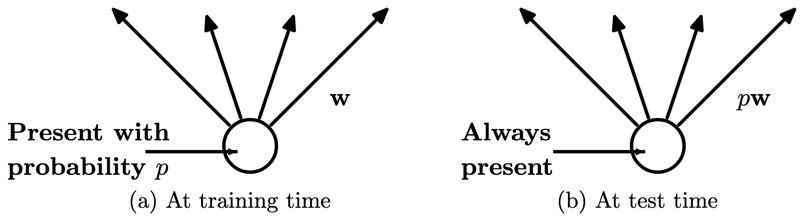
\includegraphics[width=0.6\textwidth, height=0.1\textheight, keepaspectratio]{pic/Dropout_1}
    \caption{左：训练时以概率$p$存在的单元，通过权重$\boldsymbol{w}$与下一层单元连接；右：测试时，该单元始终存在，权重 $\boldsymbol{w}$乘以$p$。测试时的输出与训练时的期望输出相同。}
    \label{fig:dropout}
\end{figure}
对于任意层$l$，$\boldsymbol{r}^{(l)}$是一个独立的随机向量，其每个元素$r_j^{(l)}$服从参数为$p$的伯努利分布。需说明的是，此处 $p$ 为神经元的\textbf{保留}概率（与原始 Dropout 论文一致，测试期对权重乘以 $p$）；而 PyTorch 的 \texttt{nn.Dropout} 及本文配置中的 $\texttt{DROPOUT\_RATE}=0.1$ 指\textbf{丢弃}概率（即 $1-p=0.1$，保留 $90\%$ 的神经元），并采用反向（inverted）Dropout——训练期对保留单元按 $1/(1-0.1)$ 放大、测试期不再缩放，二者在期望意义上等价。
向量经采样后与当前层的输出$\boldsymbol{y}^{(l)}$逐元素相乘，得到$\tilde{\boldsymbol{y}}^{(l)}$，其作为下一层的输入。
该过程在每一层均被应用，其本质是从大型网络中采样出一个子网络。

在学习阶段，损失函数的导数通过该子网络进行反向传播。测试阶段则按图\ref{fig:dropout}所示对权重进行缩放：此时神经网络以无丢弃方式运行。
\begin{figure}[H]
    \centering
    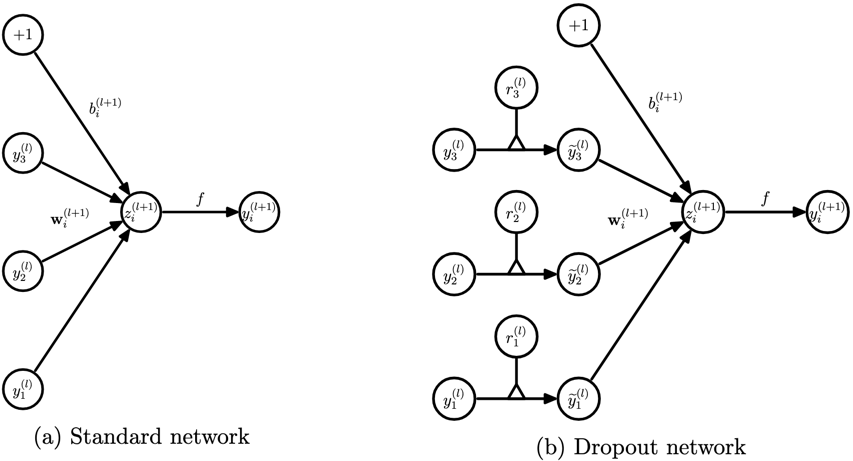
\includegraphics[width=0.8\textwidth, height=0.2\textheight, keepaspectratio]{pic/Dropout}
    \caption{标准神经网络与添加Dropout的神经网络对比图}
\end{figure}

在正向传播与权重更新过程中，标准 Dropout 以概率 $p$ 保留各神经元（即以概率 $1-p$ 暂时性地丢弃其输出及对应的连接）。
这一机制使得神经网络在每次训练迭代中都可视为一个由原网络随机采样而成的子网络，等效于在相同数据上训练大量结构略有差异的模型。

由于所有子网络共享参数并共同优化同一损失函数，最终的模型效果等价于对这些子网络预测结果的平均，从而提升了模型的稳定性与鲁棒性。
此外，Dropout 通过打破神经元之间的强依赖关系（即耦合），有效缓解了过拟合问题，增强了模型的泛化能力，显著改善了整体性能。

Dropout 在本文 ViT 模型中的应用主要体现在以下两个方面：
\begin{enumerate}[label={（\arabic*）}, leftmargin=2em, labelsep=0.5em, itemsep=0pt]
    \item 编码器中的Dropout：
    \begin{enumerate}[label={（\alph*）}, leftmargin=2em, labelsep=0.5em, itemsep=0pt]
        \item 多头注意力层中：Dropout 应用于注意力机制中 softmax 输出后的注意力权重，旨在在训练过程中以一定概率随机屏蔽部分注意力路径，从而降低模型对特定位置关系的依赖。该机制有助于抑制过拟合，提升注意力分配的鲁棒性与模型的泛化能力。
        \item 多层感知机中：Dropout 被引入至 MLP 模块中每一全连接层之后，用于在训练阶段随机丢弃部分神经元的激活输出，相当于在多个子网络之间进行模型集成。该策略有效缓解了神经元之间的共适应问题，增强了模型的正则化能力，从而提高了在未见样本上的表现。
    \end{enumerate}

    \item 解码器中的Dropout：
    \begin{enumerate}[label={（\alph*）}, leftmargin=2em, labelsep=0.5em, itemsep=0pt]
        \item 自注意力与交叉注意力层中：Dropout 同样作用于多头注意力模块中的注意力权重，分别用于解码器中处理已生成序列（自注意力）以及编码器-解码器之间的上下文建模（交叉注意力）。该机制有助于抑制注意力机制中路径依赖性过强的问题，提升模型对序列历史与图像特征之间关系的建模鲁棒性。
        \item 前馈网络中：Dropout 被用于前馈神经网络（FeedForward）模块的输出层，有效扰动神经元激活响应，降低模型在训练过程中过度拟合训练数据的风险，从而增强生成器的泛化能力。
    \end{enumerate}
\end{enumerate}

\subsubsection{早停机制}
早停机制（Early Stopping）是一种常用的正则化策略，广泛应用于深度学习模型训练过程中，旨在通过动态监控验证集上的性能表现，防止模型在训练后期出现过拟合现象。
该机制的基本思想是在模型性能不再显著提升时，自动终止训练过程，以获取最优泛化能力。其主要流程如下：
\begin{enumerate}[label={（\arabic*）}, leftmargin=2em, labelsep=0.5em, itemsep=0pt]
\item 性能监控：指定验证损失或其他评估指标作为监控对象，训练过程中持续记录模型在验证集上的性能；
\item 容忍机制：设定耐心参数（patience），允许模型在若干训练轮内性能指标未显著改善；若超过该轮数仍无改进，则认为模型已达到最优状态；
\item 权重回退：可选地在训练终止后恢复性能最优轮次对应的模型参数，以确保最终模型的泛化性能最强；
\item 资源优化：通过跳过冗余的训练轮次，能有效减少资源浪费，提升训练效率。
\end{enumerate}
综上所述，早停机制通过对模型训练过程的动态干预，实现了训练时间与模型性能之间的平衡，是提升深度学习模型泛化能力的重要技术手段之一。